% Options for packages loaded elsewhere
\PassOptionsToPackage{unicode}{hyperref}
\PassOptionsToPackage{hyphens}{url}
%
\documentclass[
]{article}
\usepackage{amsmath,amssymb}
\usepackage{lmodern}
\usepackage{iftex}
\ifPDFTeX
  \usepackage[T1]{fontenc}
  \usepackage[utf8]{inputenc}
  \usepackage{textcomp} % provide euro and other symbols
\else % if luatex or xetex
  \usepackage{unicode-math}
  \defaultfontfeatures{Scale=MatchLowercase}
  \defaultfontfeatures[\rmfamily]{Ligatures=TeX,Scale=1}
\fi
% Use upquote if available, for straight quotes in verbatim environments
\IfFileExists{upquote.sty}{\usepackage{upquote}}{}
\IfFileExists{microtype.sty}{% use microtype if available
  \usepackage[]{microtype}
  \UseMicrotypeSet[protrusion]{basicmath} % disable protrusion for tt fonts
}{}
\makeatletter
\@ifundefined{KOMAClassName}{% if non-KOMA class
  \IfFileExists{parskip.sty}{%
    \usepackage{parskip}
  }{% else
    \setlength{\parindent}{0pt}
    \setlength{\parskip}{6pt plus 2pt minus 1pt}}
}{% if KOMA class
  \KOMAoptions{parskip=half}}
\makeatother
\usepackage{xcolor}
\IfFileExists{xurl.sty}{\usepackage{xurl}}{} % add URL line breaks if available
\IfFileExists{bookmark.sty}{\usepackage{bookmark}}{\usepackage{hyperref}}
\hypersetup{
  pdftitle={Conociendo R:},
  hidelinks,
  pdfcreator={LaTeX via pandoc}}
\urlstyle{same} % disable monospaced font for URLs
\usepackage[margin=1in]{geometry}
\usepackage{color}
\usepackage{fancyvrb}
\newcommand{\VerbBar}{|}
\newcommand{\VERB}{\Verb[commandchars=\\\{\}]}
\DefineVerbatimEnvironment{Highlighting}{Verbatim}{commandchars=\\\{\}}
% Add ',fontsize=\small' for more characters per line
\usepackage{framed}
\definecolor{shadecolor}{RGB}{248,248,248}
\newenvironment{Shaded}{\begin{snugshade}}{\end{snugshade}}
\newcommand{\AlertTok}[1]{\textcolor[rgb]{0.94,0.16,0.16}{#1}}
\newcommand{\AnnotationTok}[1]{\textcolor[rgb]{0.56,0.35,0.01}{\textbf{\textit{#1}}}}
\newcommand{\AttributeTok}[1]{\textcolor[rgb]{0.77,0.63,0.00}{#1}}
\newcommand{\BaseNTok}[1]{\textcolor[rgb]{0.00,0.00,0.81}{#1}}
\newcommand{\BuiltInTok}[1]{#1}
\newcommand{\CharTok}[1]{\textcolor[rgb]{0.31,0.60,0.02}{#1}}
\newcommand{\CommentTok}[1]{\textcolor[rgb]{0.56,0.35,0.01}{\textit{#1}}}
\newcommand{\CommentVarTok}[1]{\textcolor[rgb]{0.56,0.35,0.01}{\textbf{\textit{#1}}}}
\newcommand{\ConstantTok}[1]{\textcolor[rgb]{0.00,0.00,0.00}{#1}}
\newcommand{\ControlFlowTok}[1]{\textcolor[rgb]{0.13,0.29,0.53}{\textbf{#1}}}
\newcommand{\DataTypeTok}[1]{\textcolor[rgb]{0.13,0.29,0.53}{#1}}
\newcommand{\DecValTok}[1]{\textcolor[rgb]{0.00,0.00,0.81}{#1}}
\newcommand{\DocumentationTok}[1]{\textcolor[rgb]{0.56,0.35,0.01}{\textbf{\textit{#1}}}}
\newcommand{\ErrorTok}[1]{\textcolor[rgb]{0.64,0.00,0.00}{\textbf{#1}}}
\newcommand{\ExtensionTok}[1]{#1}
\newcommand{\FloatTok}[1]{\textcolor[rgb]{0.00,0.00,0.81}{#1}}
\newcommand{\FunctionTok}[1]{\textcolor[rgb]{0.00,0.00,0.00}{#1}}
\newcommand{\ImportTok}[1]{#1}
\newcommand{\InformationTok}[1]{\textcolor[rgb]{0.56,0.35,0.01}{\textbf{\textit{#1}}}}
\newcommand{\KeywordTok}[1]{\textcolor[rgb]{0.13,0.29,0.53}{\textbf{#1}}}
\newcommand{\NormalTok}[1]{#1}
\newcommand{\OperatorTok}[1]{\textcolor[rgb]{0.81,0.36,0.00}{\textbf{#1}}}
\newcommand{\OtherTok}[1]{\textcolor[rgb]{0.56,0.35,0.01}{#1}}
\newcommand{\PreprocessorTok}[1]{\textcolor[rgb]{0.56,0.35,0.01}{\textit{#1}}}
\newcommand{\RegionMarkerTok}[1]{#1}
\newcommand{\SpecialCharTok}[1]{\textcolor[rgb]{0.00,0.00,0.00}{#1}}
\newcommand{\SpecialStringTok}[1]{\textcolor[rgb]{0.31,0.60,0.02}{#1}}
\newcommand{\StringTok}[1]{\textcolor[rgb]{0.31,0.60,0.02}{#1}}
\newcommand{\VariableTok}[1]{\textcolor[rgb]{0.00,0.00,0.00}{#1}}
\newcommand{\VerbatimStringTok}[1]{\textcolor[rgb]{0.31,0.60,0.02}{#1}}
\newcommand{\WarningTok}[1]{\textcolor[rgb]{0.56,0.35,0.01}{\textbf{\textit{#1}}}}
\usepackage{graphicx}
\makeatletter
\def\maxwidth{\ifdim\Gin@nat@width>\linewidth\linewidth\else\Gin@nat@width\fi}
\def\maxheight{\ifdim\Gin@nat@height>\textheight\textheight\else\Gin@nat@height\fi}
\makeatother
% Scale images if necessary, so that they will not overflow the page
% margins by default, and it is still possible to overwrite the defaults
% using explicit options in \includegraphics[width, height, ...]{}
\setkeys{Gin}{width=\maxwidth,height=\maxheight,keepaspectratio}
% Set default figure placement to htbp
\makeatletter
\def\fps@figure{htbp}
\makeatother
\setlength{\emergencystretch}{3em} % prevent overfull lines
\providecommand{\tightlist}{%
  \setlength{\itemsep}{0pt}\setlength{\parskip}{0pt}}
\setcounter{secnumdepth}{-\maxdimen} % remove section numbering
\ifLuaTeX
  \usepackage{selnolig}  % disable illegal ligatures
\fi

\title{Conociendo R:}
\usepackage{etoolbox}
\makeatletter
\providecommand{\subtitle}[1]{% add subtitle to \maketitle
  \apptocmd{\@title}{\par {\large #1 \par}}{}{}
}
\makeatother
\subtitle{Los primeros pasos}
\author{true}
\date{agosto 2022}

\begin{document}
\maketitle

{
\setcounter{tocdepth}{2}
\tableofcontents
}
Para regresar a Introducción R
\href{https://ciespinosa.github.io/IntroduccionR}{
\includegraphics{push1.png}}

\begin{center}\rule{0.5\linewidth}{0.5pt}\end{center}

Puedes descargar esta lección en pdf
\href{https://ciespinosa.github.io/ConociendoR/index.pdf}{aquí}

\begin{center}\rule{0.5\linewidth}{0.5pt}\end{center}

\hypertarget{por-quuxe9-usar-r}{%
\section{Por qué usar R}\label{por-quuxe9-usar-r}}

\textbf{Open source (fuente abierta)}: \textbf{R} es un lenguaje open
source, { \textbf{GRATUITO} }

\textbf{Desarrolladores}: Tiene una cantidad enorme de desarrolladores,
lo cual permite tener información y paquetes de cualquier tipo de
análisis desde SIG hasta análisis de grafos.

\textbf{Orientado a gráficos y análisis estadísticos}: R es un lenguaje
que permite desarrollar gráficos y análisis estadísticos. Tiene
capacidad para desarrollar pre-procesamiento de datos.

\textbf{Lenguaje de programación}: El hecho de que R sea un lenguaje de
programación en lugar de una colección de comandos discretos significa
que puede combinar varios comandos, cada uno usando la salida del
último, con la combinación resultante siendo bastante poderosa y
extremadamente flexible.

\hypertarget{instalando-r-y-rstudio}{%
\section{Instalando R y RStudio}\label{instalando-r-y-rstudio}}

\begin{center}\rule{0.5\linewidth}{0.5pt}\end{center}

El primer paso será instalar y . Aunque existen muchas plataformas para
trabajar con \texttt{R}, \texttt{RStudio} ofrece algunas ventajas que
las analizaremos más adelante, por las que seleccionamos esta plataforma
para trabajar.

Para instalar \texttt{R} ingresa en la página web de
\href{https://cran.r-project.org/bin/windows/base/}{r-project}. Una vez
en esta página selecciona descargar (Figura 1). Sigue los pasos para
terminar la instalación.

\begin{figure}
\centering
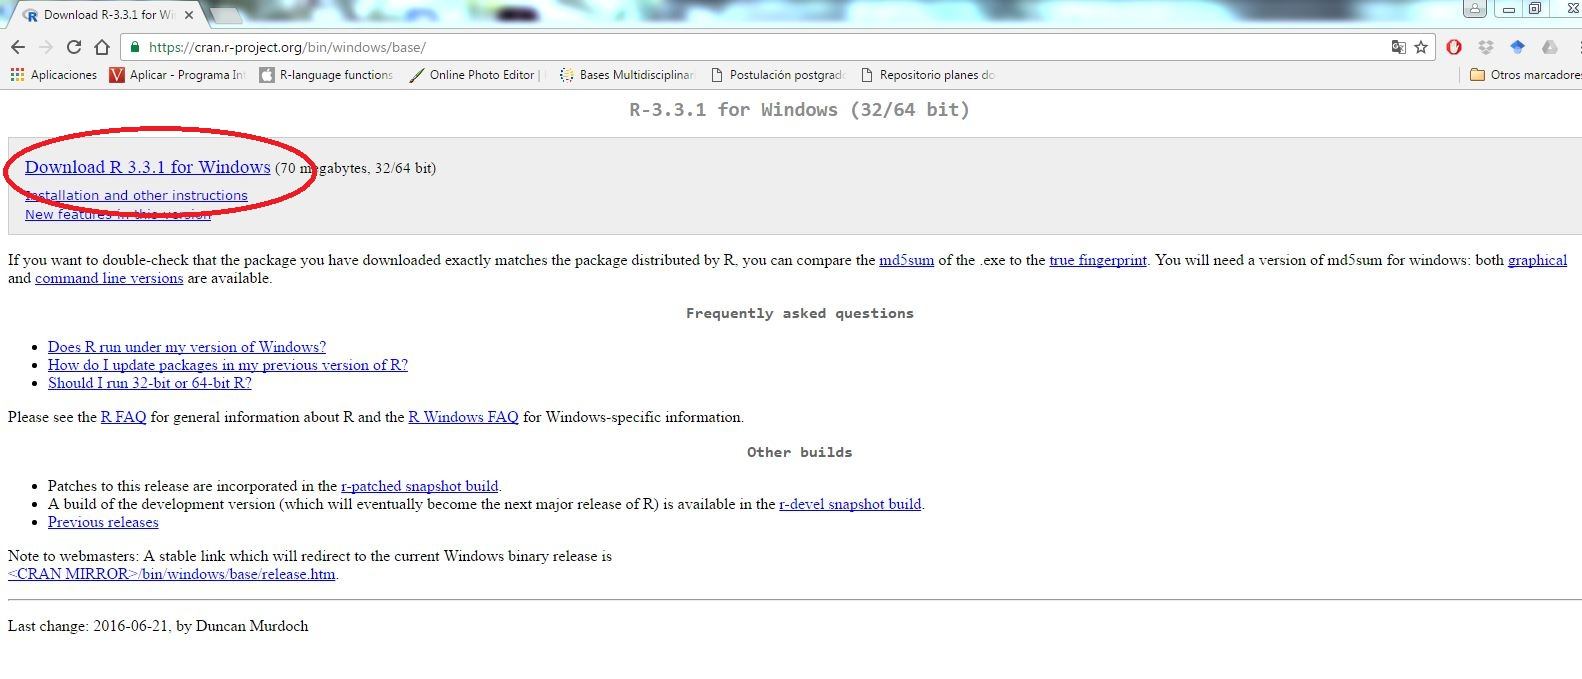
\includegraphics{imagen/descargarR.jpg}
\caption{Figura1. Descargando R}
\end{figure}

La instalación de \texttt{RStudio} es similar a R, debe ingresar en la
página de
\href{https://www.rstudio.com/products/rstudio/download/}{RStudio}. Una
vez en la página de descarga, seleccione la plataforma acorde a su
sistema operativo (Figura 2) y siga los pasos para terminar la
instalación.

\begin{figure}
\centering
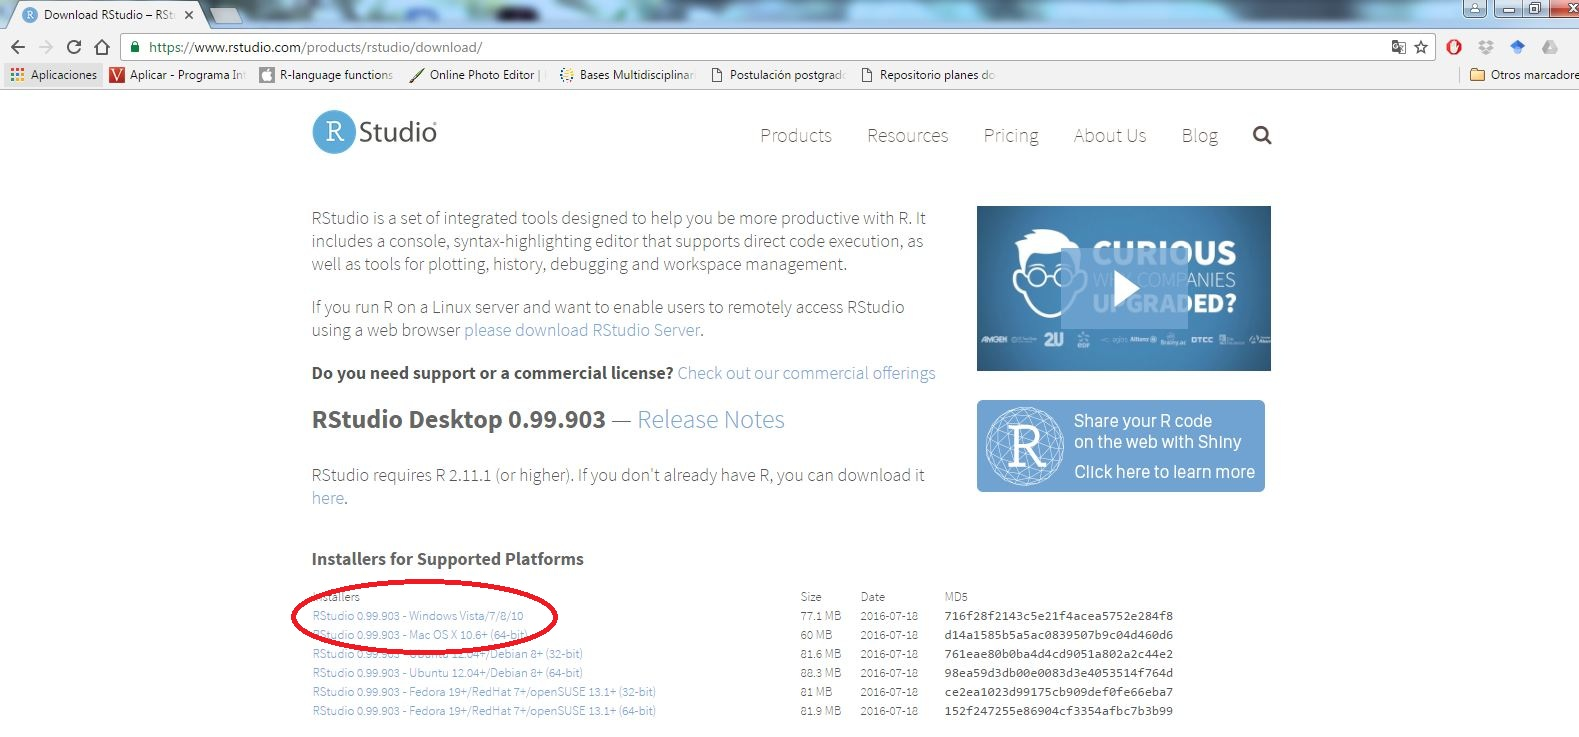
\includegraphics{imagen/descargarRStudio.jpg}
\caption{Figura2. Descargando RStudio}
\end{figure}

Una vez que hemos instalado R y RStudio podremos trabajar con los datos.
Una cosa importante es que RStudio no puede funcionar si no hemos
descargado R, así que se debe asegurar descargar los dos programas.
Trabajaremos en RStudio así que no es necesario que despliegue R.

\begin{quote}
Nota: ``El uso de comandos exige una curva de aprendizaje mayor que el
requerido por las interfaces gráficas, pero las ganancias en términos de
independencia, creatividad y control no son comparables. Escribir un
código supone una comprensión más profunda de aquello que se desea
aplicar'' (Elousa 2011).
\end{quote}

\begin{center}\rule{0.5\linewidth}{0.5pt}\end{center}

\#Conozcamos RStudio antes de empezar

\begin{figure}
\centering
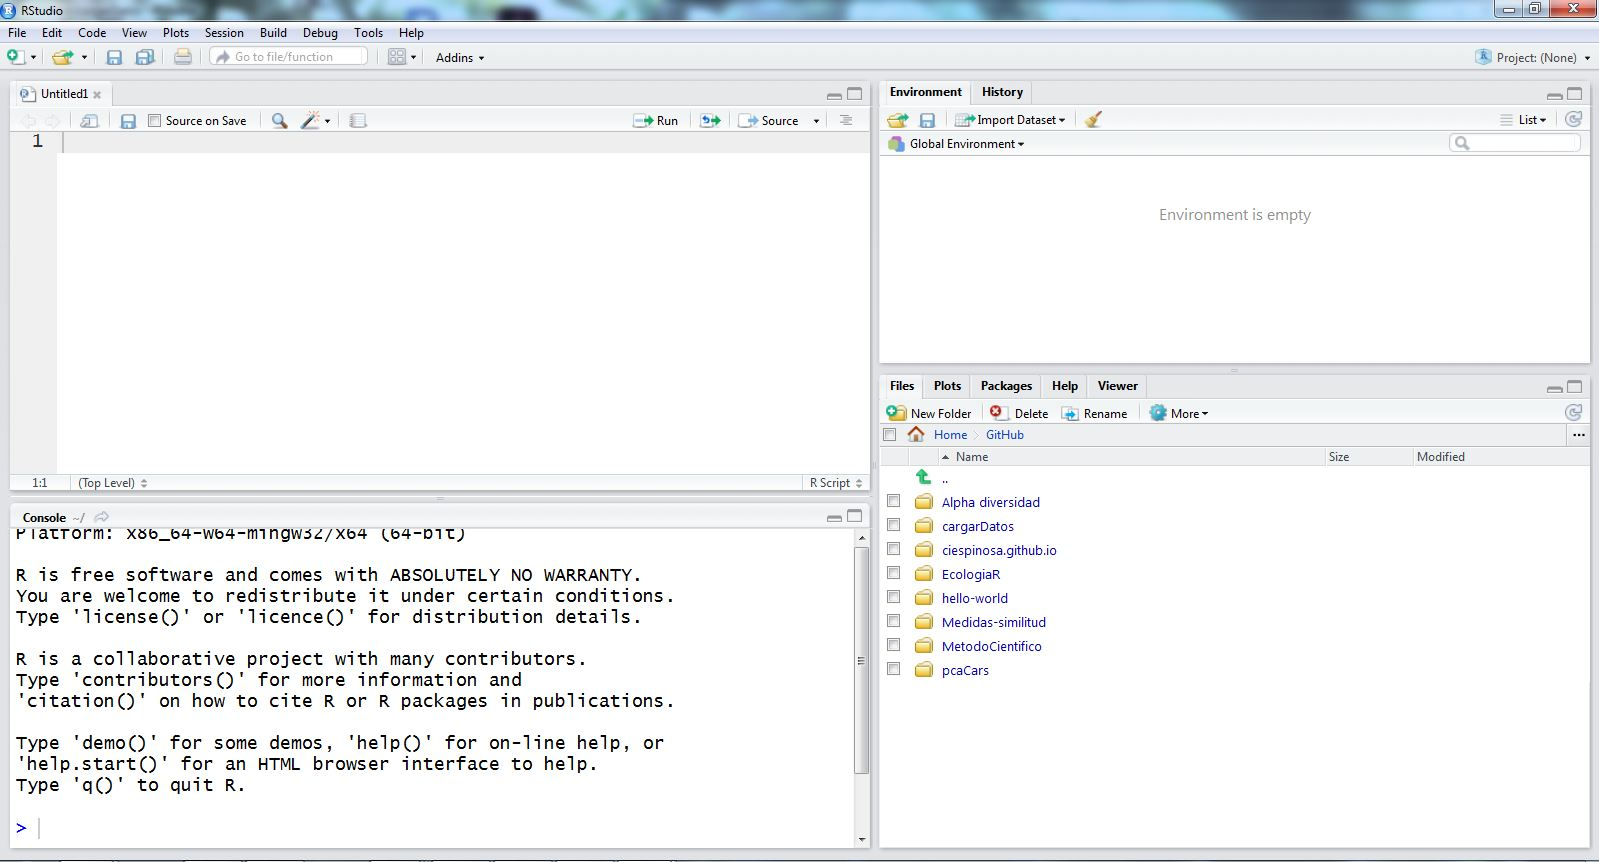
\includegraphics{imagen/RStudio.jpg}
\caption{Figura 4. Plataforma RStudio}
\end{figure}

Como vemos en la figura 4, RStudio está compuesto por cuatro ventanas.
Seguramente en su caso, si acaba de abrir RStudio le aparecerán
únicamente tres ventanas. A continuación, describiré cada una de las
ventanas.

La \textbf{primera ventana} (la que en su caso seguramente no tiene,
izquierda superior) lo constituye documentos que pueden ser de varios
tipos. El tipo básico es un documento con extensión \textbf{.R}, el cual
sirve para guardar el código desarrollado para el análisis. Vamos abrir
un documento .R (script), esto lo podemos hacer de al menos tres
maneras, la primera es ir al menú de la consola seleccionar
\texttt{File\ \textgreater{}\ New\ File\ \textgreater{}\ script}, la
segunda forma es seleccionar el icono del documento con una cruz verde

\includegraphics{imagen/RStudio_nuevo.jpg} y seleccionar
\texttt{R\ script}. La última opción es hacerlo desde el teclado,
presione \texttt{alt\ +\ shift} (mayúsculas) y la tecla \textbf{N}
obtendrá el mismo resultado.

Existen otros muchos archivos que podemos cargar, pero por ahora veremos
solo este.

La \textbf{segunda ventana} (derecha superior), esta ventana se verán
todos los objetos que iremos cargando o generando durante el trabajo en
RStudio, por ahora esta ventana estará vacía. Esta ventana nos muestra
la memoria activa de R, lo que en un computador se conoce como la
memoria RAM.

\begin{quote}
Vamos a generar algunos objetos y ver lo que pasa.
\end{quote}

\begin{Shaded}
\begin{Highlighting}[]
\NormalTok{nombre}\OtherTok{\textless{}{-}} \StringTok{"Carlos Ivan"}
\NormalTok{apellido}\OtherTok{\textless{}{-}} \StringTok{"Espinosa Iñiguez"}
\NormalTok{matriz}\OtherTok{\textless{}{-}} \FunctionTok{matrix}\NormalTok{(}\DecValTok{1}\SpecialCharTok{:}\DecValTok{20}\NormalTok{, }\DecValTok{5}\NormalTok{,}\DecValTok{4}\NormalTok{)}
\end{Highlighting}
\end{Shaded}

Ahora podemos ver los objetos creados, algunos salen como valores y la
matriz sale como datos. Los objetos pueden ser abiertos para ver su
estructura. Si hacen clic en el nombre matriz verán que se abre una
nueva hoja en la primera ventana que corresponde a estos datos.

La \textbf{tercera ventana} (izquierda abajo), corresponde a la consola
de R, esta es la consola donde se ejecutarán todos los códigos y se
realizarán los análisis. Esta ventana es R. RStudio incorpora a R dentro
de su ejecución, por lo que si no hemos instalado R esta ventana no
aparecerá.

La \textbf{cuarta ventana} (derecha abajo), en esta ventana tenemos
varias pestañas. La primera \texttt{File} nos muestra todos los archivos
que están en la carpeta de mi proyecto, guardados en el disco duro.
Pueden ser archivos de datos, gráficos generados o el script de R que
estoy generando. La siguiente pestaña \texttt{Plots} mostrará los
gráficos que va ejecutando en R. La pestaña \texttt{Help} puede ser
usada para pedir ayuda de algún paquete o función que necesite usar, y
no esté claro de cómo hacerlo.

Bueno ya conocemos RStudio ahora si a trabajar.

\begin{quote}
Nota: El trabajar con códigos requiere que seamos ordenados y
sistemáticos, de no cumplir estos requerimientos tendrá un verdadero
dolor de cabeza. RStudio es una interesante plataforma que nos permite
organizar el trabajo. Siempre que inician un trabajo de análisis siga
los pasos propuestos a continuación.
\end{quote}

\begin{center}\rule{0.5\linewidth}{0.5pt}\end{center}

\hypertarget{los-primeros-pasos}{%
\section{Los primeros pasos}\label{los-primeros-pasos}}

El trabajo de programación requiere ser ordenados, considero que
trabajar con RStudio nos ofrece algunas ventajas para organizar ese
trabajo.

\hypertarget{primer-paso-crear-un-proyecto}{%
\subsection{Primer Paso: Crear un
proyecto}\label{primer-paso-crear-un-proyecto}}

Crear un proyecto implica definir un directorio desde el cual \texttt{R}
funcionará. Este proceso creará una carpeta a la cual R estará anclado.
Además, en esta carpetaencontrará un archivo .Rproj desde el cual podrá
abrir RStudio.

Para crear un nuevo proyecto en RStudio debemos seguir los siguientes
pasos.

\begin{enumerate}
\def\labelenumi{\arabic{enumi}.}
\tightlist
\item
  Abrir RStudio
\item
  Hacer clic en \texttt{file} y seleccionar new \texttt{Project}
\item
  En la nueva ventana que se abrió, podemos seleccionar entre tres
  opciones, puesto que aún no estamos trabajando con versiones de
  control, por ahora podemos seleccionar entre nuevo directorio
  \texttt{New\ Directory} o un directorio existente
  \texttt{Existing\ Directory}.
\end{enumerate}

Si seleccionamos \texttt{New\ Directory}(nuevo directorio) se generará
una nueva carpeta en la ubicación que nosotros definamos, en esta
carpeta podremos poner todos los datos y demás información con la cual
trabajaremos. Cuando seleccionamos \texttt{Existing\ Directory} (un
directorio existente) RStudio generará un proyecto dentro de una carpeta
que ya exista en el computador. Por organización, siempre que estoy
iniciando un nuevo proyecto prefiero crear un nuevo directorio en el
cual colocaré únicamente los archivos que voy a utilizar en los
análisis.

\begin{enumerate}
\def\labelenumi{\arabic{enumi}.}
\setcounter{enumi}{3}
\item
  Si hemos elegido \texttt{New\ Directory} tendremos dos casilleros, el
  primero indica el nombre que le vamos a poner a la carpeta
  \texttt{Directory\ Name} y el segundo nos indica donde alojaremos esa
  carpeta \texttt{browse}.
\item
  Si hemos elegido \texttt{Existing\ Directory}, la siguiente ventana
  nos permite decir cuál es la carpeta que quiero enlazar. Hacer clic en
  \texttt{browse} buscar la carpeta donde colocaré el proyecto y
  aceptar.
\end{enumerate}

\#\#Segundo Paso: Los códigos usados

Si bien podemos trabajar directamente en la consola de R para ejecutar
los códigos, lo mejor es que desde el principio nos acostumbremos a
generar scripts, donde tengamos la información limpia y podamos saber lo
que estamos haciendo. Un Script es un archivo donde tendremos los
códigos de R, referenciados y organizados.

\textbf{Algunos consejos iniciales}

\begin{enumerate}
\def\labelenumi{\alph{enumi}.}
\item
  Todos los códigos usados para realizar los diferentes análisis, deben
  siempre deben ir acompañados de una nota que explique lo que están
  haciendo. La nota debe estar precedida por \textbf{\#}, con lo cual R
  no lee esta parte como código (Figura 4).
\item
  Recuerden siempre colocar sus archivos de datos en la carpeta del
  proyecto que generaron en el primer paso.
\item
  Si está probando cambios en el código, una vez que tiene un código que
  funciona, borre el código con error o que no le funcionó, tenga
  siempre su código limpio.
\item
  Una vez que escribe el código, este puede ser ejecutado desde la
  consola haciendo clic en la consola en el ícono run
  
\includegraphics{imagen/RStudio_Run.jpg} que se encuentra en la parte
  superior derecha de la ventana del script. Sin embargo, una mejor
  forma es tecleando \textbf{ctrl} y \textbf{enter}.
\item
  Cada vez que en el código iniciamos un nuevo tema, podemos poner un
  título seguido por cuatro guiones medios (- - - -), esto genera en
  RStudio una estructura de índice que puede ser navegada (Figura 5
  círculo rojo abajo a la izquierda).
\end{enumerate}

\begin{figure}
\centering
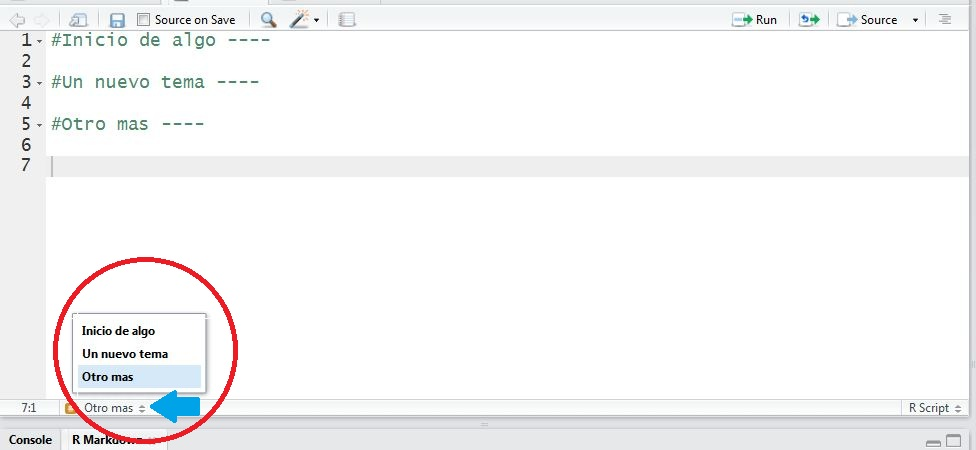
\includegraphics{imagen/estructura.jpg}
\caption{Figura 5. Estructura del script en RStudio}
\end{figure}

\begin{quote}
Nota: Es importante que sea organizado en la ejecución de los códigos,
siga los consejos y podrá mantener un código limpio y fácil de acceder y
revisar.
\end{quote}

\begin{center}\rule{0.5\linewidth}{0.5pt}\end{center}

\hypertarget{el-funcionamiento-de-r}{%
\section{El funcionamiento de R}\label{el-funcionamiento-de-r}}

Hemos hablado mucho de \texttt{R} pero hasta ahora no hemos dicho que
es, ¿es un programa?, no, realmente no es un programa, es un entorno de
programación. R es considerado un dialecto del lenguaje \emph{S} el cual
fue desarrollado por los Laboratorios AT\&T Bell.

Aunque mucha gente se asusta cuando hablamos de R, como un lenguaje de
programación, la realidad es que R es un lenguaje bastante simple, está
orientado a \emph{Objetos}. Por otro lado, a diferencia de otros
lenguajes de programación los comandos escritos en el teclado, son
ejecutados directamente sin necesidad de construir ejecutables.

En R tenemos al menos tres grandes categorías de objetos; funciones,
datos y resultados. Cada una de estas tiene unas características
propias. Las \emph{funciones} normalmente se encuentran dentro de
paquetes, estos objetos traen comandos que permiten manipular los datos.
Accedemos a las funciones a través de comandos. Los \emph{datos} son
matrices o vectores de información los cuales son manipulados por las
funciones. Los \emph{resultados} son objetos resultantes de la
manipulación de los datos (Figura 3).

\begin{figure}

{\centering \includegraphics{index_files/figure-latex/unnamed-chunk-2-1} 

}

\caption{Figura 3. Esquema del funcionamiento de r. Basado en Paradis 2003}\label{fig:unnamed-chunk-2}
\end{figure}

El funcionamiento de R se da en la memoria activa, así que cada vez que
iniciamos a trabajar con R es necesario llamar los datos desde el disco
duro a la memoria activa. Para llamar paquetes (donde tenemos las
funciones) normalmente utilizamos la función \texttt{library}, mientras
que para llamar los datos utilizamos funciones como \texttt{read.table}.
Algunas veces nos interesa grabar un resultado desde la memoria activa
al disco duro para esto podemos utilizar funciones como
\texttt{write.table}. Finalmente, no todos los paquetes disponibles se
bajan cuando instalamos R, de hecho, solo se baja un paquete conocido
como paquete base. Cuando se necesita un nuevo paquete, este debe
llamarse desde internet, para ello utilizamos la función
\texttt{install.packages}. Existe un repositorio de todos los paquetes
disponibles (Comprehensive R Archive Network, \textbf{CRAN}) y varios
países tienen espejos de estos repositorios (espejos CRAN) a partir de
los cuales podemos descargar los paquetes.

\begin{quote}
Nota: Es muy importante que antes de empezar a trabajar con R seamos
conscientes de cómo funciona, esto facilitará entender lo que está
haciendo cuando introduce un código.
\end{quote}

\begin{center}\rule{0.5\linewidth}{0.5pt}\end{center}

\hypertarget{uso-de-la-memoria-activa}{%
\subsection{Uso de la memoria activa}\label{uso-de-la-memoria-activa}}

Vamos a trabajar en R

\begin{enumerate}
\def\labelenumi{\arabic{enumi}.}
\tightlist
\item
  Abra RStudio y cree un proyecto
\item
  Genere un Script para escribir el código.
\item
  Ahora a trabajar
\end{enumerate}

\begin{center}\rule{0.5\linewidth}{0.5pt}\end{center}

\hypertarget{ejecuciuxf3n-de-comandos-e-impresiuxf3n}{%
\subsubsection{Ejecución de comandos e
impresión}\label{ejecuciuxf3n-de-comandos-e-impresiuxf3n}}

Cuando estamos trabajando con R, nosotros podemos desarrollar una serie
de acciones u operaciones que se ejecutan en la consola, luego de lo
cual el resultado puede ser impreso en la consola. Veamos unos ejemplos.

\begin{Shaded}
\begin{Highlighting}[]
\CommentTok{\#Ejecución de comandos e impresión}

\NormalTok{pi}\SpecialCharTok{*}\DecValTok{3}
\end{Highlighting}
\end{Shaded}

\begin{verbatim}
## [1] 9.424778
\end{verbatim}

\begin{Shaded}
\begin{Highlighting}[]
\FunctionTok{log}\NormalTok{(}\DecValTok{234}\NormalTok{)}
\end{Highlighting}
\end{Shaded}

\begin{verbatim}
## [1] 5.455321
\end{verbatim}

Cuando nosotros introducimos el comando en R y lo ejecutamos, podemos
ver la salida de esa expresión, R imprime el resultado directamente en
la consola. Podemos usar la función \texttt{print()} para pedir a R que
imprima el resultado.

\begin{Shaded}
\begin{Highlighting}[]
\DocumentationTok{\#\#La función de impresión}

\FunctionTok{print}\NormalTok{(pi}\SpecialCharTok{*}\DecValTok{3}\NormalTok{); }\FunctionTok{print}\NormalTok{(pi}\SpecialCharTok{*}\DecValTok{3}\NormalTok{, }\AttributeTok{digits =} \DecValTok{4}\NormalTok{) }\CommentTok{\#El ; nos permite separar dos líneas de código}
\end{Highlighting}
\end{Shaded}

\begin{verbatim}
## [1] 9.424778
\end{verbatim}

\begin{verbatim}
## [1] 9.425
\end{verbatim}

\begin{Shaded}
\begin{Highlighting}[]
\FunctionTok{print}\NormalTok{(}\FunctionTok{log}\NormalTok{(}\DecValTok{234}\NormalTok{), }\AttributeTok{digits =} \DecValTok{10}\NormalTok{)}
\end{Highlighting}
\end{Shaded}

\begin{verbatim}
## [1] 5.455321115
\end{verbatim}

Como vemos con el uso de la función \texttt{print()} tenemos la misma
salida, imprime el resultado en la consola. Sin embargo, nos permite
cambiar ciertas propiedades de lo que se imprime, en este caso controlar
el número de decimales. Cuando trabajamos con tablas, la función print
nos permite controlar la salida de esas tablas.

\begin{Shaded}
\begin{Highlighting}[]
\DocumentationTok{\#\#Controlar la salida de tablas}

\FunctionTok{print}\NormalTok{(}\FunctionTok{as.table}\NormalTok{(}\FunctionTok{matrix}\NormalTok{(}\FunctionTok{c}\NormalTok{(}\DecValTok{5}\SpecialCharTok{:}\DecValTok{0}\NormalTok{,}\DecValTok{1}\NormalTok{,}\DecValTok{0}\NormalTok{,}\DecValTok{0}\NormalTok{),}\DecValTok{3}\NormalTok{,}\DecValTok{3}\NormalTok{)))}
\end{Highlighting}
\end{Shaded}

\begin{verbatim}
##   A B C
## A 5 2 1
## B 4 1 0
## C 3 0 0
\end{verbatim}

\begin{Shaded}
\begin{Highlighting}[]
\FunctionTok{print}\NormalTok{(}\FunctionTok{as.table}\NormalTok{(}\FunctionTok{matrix}\NormalTok{(}\FunctionTok{c}\NormalTok{(}\DecValTok{5}\SpecialCharTok{:}\DecValTok{0}\NormalTok{,}\DecValTok{1}\NormalTok{,}\DecValTok{0}\NormalTok{,}\DecValTok{0}\NormalTok{),}\DecValTok{3}\NormalTok{,}\DecValTok{3}\NormalTok{)), }\AttributeTok{zero.print =} \StringTok{"."}\NormalTok{)}
\end{Highlighting}
\end{Shaded}

\begin{verbatim}
##   A B C
## A 5 2 1
## B 4 1 .
## C 3 . .
\end{verbatim}

En este caso el argumento \emph{zero.print} nos permite decirle que
queremos substituir los ceros por un punto podemos cambiar el punto por
un ``-''. Inténtalo y mira lo que obtienes.

Aunque la función print nos permite tener cierto control sobre lo que
imprimimos en la consola, esta función solo puede ser aplicada a una
expresión a la vez. Cuando queremos que se imprima una expresión
compuesta por varias expresiones, podemos usar la función \texttt{cat()}

\begin{Shaded}
\begin{Highlighting}[]
\DocumentationTok{\#\#La función cat para imprimir vectores}

\FunctionTok{cat}\NormalTok{(}\StringTok{"Juan tiene"}\NormalTok{, }\FunctionTok{round}\NormalTok{(}\DecValTok{17}\SpecialCharTok{*}\NormalTok{pi, }\DecValTok{2}\NormalTok{), }\StringTok{"años}\SpecialCharTok{\textbackslash{}n}\StringTok{"}\NormalTok{, }
    \StringTok{"Juan es adulto mayor"}\NormalTok{)}
\end{Highlighting}
\end{Shaded}

\begin{verbatim}
## Juan tiene 53.41 años
##  Juan es adulto mayor
\end{verbatim}

La función \textbf{cat} permite imprimir varias cosas juntas, intente
usar la expresión print para ejecutar el mismo vector. ¿Qué sucedió?. El
argumento final \textbf{``\n''} nos dice que hay un salto de línea.

Hasta aquí, todos los códigos que hemos ejecutado se han impreso en la
consola pero no constan en ningún lado, todos los resultados de esos
códigos no pueden ser usados para realizar ninguna otra acción. Hemos
usado R como una calculadora, la cual nos da un resultado, pero no
podemos volver a acceder a ese resultado de ninguna forma.

Para acceder a los resultados necesitamos asignar el resultado a un
símbolo, un nombre.

\hypertarget{asignaciuxf3n-y-generaciuxf3n-de-objetos}{%
\subsubsection{Asignación y generación de
objetos}\label{asignaciuxf3n-y-generaciuxf3n-de-objetos}}

El trabajo que hicimos en la sección anterior no generó objetos, como
había comentado los objetos son las estructuras sobra las cuales R
opera. Podemos generar objetos usando la función \texttt{\textless{}-}.
Existen otras formas de asignar, como ``='', o ``-\textgreater{}'', sin
embargo, es mejor no usarlas puesto que por ejemplo el ``='' puede ser
confundida con la expresión \emph{igual que}. En el caso de la función
``-\textgreater{}'' si bien cuando generamos un objeto sencillo puede
usarse, cuando estamos generando una expresión más compleja es muy
difícil entender si al final está la asignación. Por estas razones es
mejor que siempre use ``\textless-''.

\textbf{Trabajemos nuevamente en R}

\begin{Shaded}
\begin{Highlighting}[]
\DocumentationTok{\#\#Asignando resultados a símbolos}
\FunctionTok{set.seed}\NormalTok{(}\DecValTok{23}\NormalTok{)}
\NormalTok{edad }\OtherTok{\textless{}{-}} \FunctionTok{round}\NormalTok{(}\FunctionTok{rnorm}\NormalTok{(}\DecValTok{5}\NormalTok{, }\DecValTok{25}\NormalTok{,}\DecValTok{40}\NormalTok{),}\DecValTok{2}\NormalTok{)}
\end{Highlighting}
\end{Shaded}

\emph{\textbf{Un momento, algo paso, no veo el resultado.}}

Puede chequear el ``Environment'' en RStudio, ¿qué puede ver ahí?.
Efectivamente, aparece el nombre edad. Hemos generado un objeto que está
representado por el símbolo \emph{edad}

Usar la función asignar ``\textless-'', y hemos asignado el resultado de
nuestro código a un símbolo (nombre). R reconoce este nombre como un
símbolo, es por eso que \textbf{Edad} no es lo mismo que \textbf{edad}.

Ahora, ¿cómo podemos imprimir el resultado de edad?. Ejecutando las
mismas funciones de imprimir (print y cat) que usamos antes o teclear
directamente el nombre.

\begin{Shaded}
\begin{Highlighting}[]
\CommentTok{\#Imprimir los objetos}
\FunctionTok{print}\NormalTok{(edad)}
\end{Highlighting}
\end{Shaded}

\begin{verbatim}
## [1] 32.73  7.61 61.53 96.74 64.86
\end{verbatim}

\begin{Shaded}
\begin{Highlighting}[]
\NormalTok{edad}
\end{Highlighting}
\end{Shaded}

\begin{verbatim}
## [1] 32.73  7.61 61.53 96.74 64.86
\end{verbatim}

Vamos a jugar un poco. Usaremos la \texttt{función\ cat()} para imprimir
un objeto que tiene varios elementos, imprimiremos cada uno de los
elementos que están asociados. En este caso tenemos un nombre de una
persona y la edad de esas personas. Para esto usamos una función que
genera un loop (un proceso circular un bucle), en este caso la función
\texttt{for()}. Esta función permite definir un símbolo en este caso
``i'' y darle un valor secuencial definido por el usuario. En el caso
del ejemplo i tomará los valores de 1 a 5 (número de elementos en nom),
de esta forma R generará un ciclo (bucle) en el cual \emph{i} toma el
valor de \emph{1}, en la siguiente vuelta \emph{2} y así sucesivamente
hasta 5.

\begin{Shaded}
\begin{Highlighting}[]
\CommentTok{\#Vector de nombres}

\NormalTok{nom }\OtherTok{\textless{}{-}} \FunctionTok{c}\NormalTok{(}\StringTok{"Juan"}\NormalTok{, }\StringTok{"Pedro"}\NormalTok{, }\StringTok{"Ana"}\NormalTok{, }\StringTok{"Sol"}\NormalTok{, }\StringTok{"Juliana"}\NormalTok{)}

\CommentTok{\#Usamos la función cat para imprimir}

\ControlFlowTok{for}\NormalTok{(i }\ControlFlowTok{in} \DecValTok{1}\SpecialCharTok{:}\FunctionTok{length}\NormalTok{(nom)) }\FunctionTok{cat}\NormalTok{(}\StringTok{"La edad de"}\NormalTok{, nom[i], }\StringTok{"es"}\NormalTok{, edad[i], }\StringTok{"}\SpecialCharTok{\textbackslash{}n}\StringTok{"}\NormalTok{)}
\end{Highlighting}
\end{Shaded}

\begin{verbatim}
## La edad de Juan es 32.73 
## La edad de Pedro es 7.61 
## La edad de Ana es 61.53 
## La edad de Sol es 96.74 
## La edad de Juliana es 64.86
\end{verbatim}

Pero, no sabemos que categoría tiene. Podemos incluir la categoría de
joven, adulto o adulto mayor. Usaremos la función ´if()´ para pedirle a
R que nos diga que categoría tiene cada uno.

\begin{Shaded}
\begin{Highlighting}[]
\CommentTok{\#Vector de nombres}

\NormalTok{nom }\OtherTok{\textless{}{-}} \FunctionTok{c}\NormalTok{(}\StringTok{"Juan"}\NormalTok{, }\StringTok{"Pedro"}\NormalTok{, }\StringTok{"Ana"}\NormalTok{, }\StringTok{"Sol"}\NormalTok{, }\StringTok{"Juliana"}\NormalTok{)}

\CommentTok{\#Usamos la función cat para imprimir}

\ControlFlowTok{for}\NormalTok{(i }\ControlFlowTok{in} \DecValTok{1}\SpecialCharTok{:}\FunctionTok{length}\NormalTok{(nom)) }\FunctionTok{cat}\NormalTok{(}\StringTok{"La edad de"}\NormalTok{, nom[i], }\StringTok{"es"}\NormalTok{, edad[i], }\StringTok{"}\SpecialCharTok{\textbackslash{}n}\StringTok{"}\NormalTok{,}
\NormalTok{                            nom[i], }\StringTok{"es un"}\NormalTok{, }\FunctionTok{ifelse}\NormalTok{(edad[i]}\SpecialCharTok{\textless{}}\DecValTok{20}\NormalTok{, }\StringTok{"joven"}\NormalTok{, }
                                               \FunctionTok{ifelse}\NormalTok{(edad[i]}\SpecialCharTok{\textgreater{}}\DecValTok{50}\NormalTok{, }\StringTok{"adulto mayor"}\NormalTok{, }\StringTok{"adulto"}\NormalTok{)), }\StringTok{"}\SpecialCharTok{\textbackslash{}n}\StringTok{"}\NormalTok{)}
\end{Highlighting}
\end{Shaded}

\begin{verbatim}
## La edad de Juan es 32.73 
##  Juan es un adulto 
## La edad de Pedro es 7.61 
##  Pedro es un joven 
## La edad de Ana es 61.53 
##  Ana es un adulto mayor 
## La edad de Sol es 96.74 
##  Sol es un adulto mayor 
## La edad de Juliana es 64.86 
##  Juliana es un adulto mayor
\end{verbatim}

En esta segunda parte hemos trabajado en la memoria activa de la
computadora, la memoria RAM. Cuando asignamos una variable a un símbolo,
como en este caso ``edad'', la variable se mantiene en su espacio de
trabajo (Workspace). El espacio de trabajo se mantiene en la memoria
activa de la computadora, pero se puede guardar en el disco cuando R se
cierra. La variable permanece en el espacio de trabajo hasta que el
usuario la elimine. Aunque, RStudio permite ver el workspace, podemos
pedirle a R que nos muestre lo que tiene en su ``workspace'' usando la
función \texttt{ls()}.

\begin{Shaded}
\begin{Highlighting}[]
\CommentTok{\#Listado del workspace}
\FunctionTok{ls}\NormalTok{()}
\end{Highlighting}
\end{Shaded}

\begin{verbatim}
## [1] "apellido" "edad"     "i"        "matriz"   "nom"      "nombre"   "x"       
## [8] "y"
\end{verbatim}

Podemos pedir que nos diga las características de esos objetos

\begin{Shaded}
\begin{Highlighting}[]
\CommentTok{\#listado con características}

\FunctionTok{ls.str}\NormalTok{()}
\end{Highlighting}
\end{Shaded}

\begin{verbatim}
## apellido :  chr "Espinosa Iñiguez"
## edad :  num [1:5] 32.73 7.61 61.53 96.74 64.86
## i :  int 5
## matriz :  int [1:5, 1:4] 1 2 3 4 5 6 7 8 9 10 ...
## nom :  chr [1:5] "Juan" "Pedro" "Ana" "Sol" "Juliana"
## nombre :  chr "Carlos Ivan"
## x :  int [1:100] 1 2 3 4 5 6 7 8 9 10 ...
## y :  int [1:100] 1 2 3 4 5 6 7 8 9 10 ...
\end{verbatim}

\hypertarget{eliminando-objetos}{%
\subsubsection{Eliminando objetos}\label{eliminando-objetos}}

Puede ser que necesite borrar algunos objetos que ya no ocuparé, para
ello usaremos la función \texttt{rm()}. Veamos cómo lo podemos hacer.

\begin{Shaded}
\begin{Highlighting}[]
\FunctionTok{ls}\NormalTok{(); }\FunctionTok{rm}\NormalTok{(i); }\FunctionTok{ls}\NormalTok{()}
\end{Highlighting}
\end{Shaded}

\begin{verbatim}
## [1] "apellido" "edad"     "i"        "matriz"   "nom"      "nombre"   "x"       
## [8] "y"
\end{verbatim}

\begin{verbatim}
## [1] "apellido" "edad"     "matriz"   "nom"      "nombre"   "x"        "y"
\end{verbatim}

Como ven en la primera salida de nuestro workspce consta ``i'', pero la
segunda vez que ejecutamos ls el objeto ``i'' ya no aparece.

Podemos usar la expresión rm(list=ls()) para borrar todos los objetos en
el workspace o usar la expresión rm(list=setdiff(ls(), c(``edad'',
``nom''))), para eliminar todo aquello que no sea ``edad'' ni ``nom''

\begin{center}\rule{0.5\linewidth}{0.5pt}\end{center}

\hypertarget{uso-del-disco-duro}{%
\subsection{Uso del disco duro}\label{uso-del-disco-duro}}

Hasta ahora hemos trabajado en la memoria activa, eso quiere decir, que
cuando cerremos R todos los objetos que hemos desarrollado se pierden.
Es posible que eso sea lo que quiero, pero seguramente hay resultados
que me gustaría grabar en mi disco duro para poder acceder a ellos.

A diferencia de programas tradicionales, para grabar los datos necesito
usar una función y no un menu de ventanas.

\hypertarget{guardando-datos}{%
\subsubsection{Guardando datos}\label{guardando-datos}}

Podemos usar la función \textbf{sink} para redireccionar la salida a un
archivo .txt, de esta forma, R ya no imprimirá en la consola sino que lo
hará en el documento que hemos generado. Debemos volver a correr la
función \textbf{sink} para que se cierre la conexión con el archivo.

\textbf{Recuerden:} siempre deben cerrar esta función caso contrario
todo lo que hagan se imprimirá en este archivo.

\begin{Shaded}
\begin{Highlighting}[]
\FunctionTok{sink}\NormalTok{(}\StringTok{"names\_output.txt"}\NormalTok{)}
\ControlFlowTok{for}\NormalTok{(i }\ControlFlowTok{in} \DecValTok{1}\SpecialCharTok{:}\FunctionTok{length}\NormalTok{(nom)) }\FunctionTok{cat}\NormalTok{(}\StringTok{"La edad de"}\NormalTok{, nom[i], }\StringTok{"es"}\NormalTok{, edad[i], }\StringTok{"...}\SpecialCharTok{\textbackslash{}n}\StringTok{"}\NormalTok{)}
\FunctionTok{sink}\NormalTok{()}
\end{Highlighting}
\end{Shaded}

Podríamos generar un reporte con los datos utilizando la función
\textbf{sink}. De esta forma, procesaremos los datos de edad y género
que tenemos y los imprimiremos en un \textbf{.txt} llamado reporte1.

\begin{Shaded}
\begin{Highlighting}[]
\NormalTok{dta }\OtherTok{\textless{}{-}} \FunctionTok{data.frame}\NormalTok{(edad, nom, }\AttributeTok{gen=}\FunctionTok{c}\NormalTok{(}\FunctionTok{rep}\NormalTok{(}\StringTok{"Hombres"}\NormalTok{,}\DecValTok{2}\NormalTok{), }\FunctionTok{rep}\NormalTok{(}\StringTok{"Mujeres"}\NormalTok{,}\DecValTok{3}\NormalTok{)))}
\NormalTok{resul }\OtherTok{\textless{}{-}} \FunctionTok{tapply}\NormalTok{(dta}\SpecialCharTok{$}\NormalTok{edad, dta}\SpecialCharTok{$}\NormalTok{gen, mean)}
\end{Highlighting}
\end{Shaded}

\begin{Shaded}
\begin{Highlighting}[]
\FunctionTok{sink}\NormalTok{(}\StringTok{"reporte1.txt"}\NormalTok{)}

\FunctionTok{print}\NormalTok{(resul)}

\FunctionTok{summary}\NormalTok{(dta)}
\FunctionTok{cat}\NormalTok{(}\StringTok{"Conclusión: La mayor media de edad se presenta en"}\NormalTok{,}
    \FunctionTok{names}\NormalTok{(resul[resul}\SpecialCharTok{==}\FunctionTok{max}\NormalTok{(resul)]),}\StringTok{"("}\NormalTok{, }\FunctionTok{max}\NormalTok{(resul), }\StringTok{")"}\NormalTok{, }
     \StringTok{", mientras que la menor edad en"}\NormalTok{, }
    \FunctionTok{names}\NormalTok{(resul[resul}\SpecialCharTok{==}\FunctionTok{min}\NormalTok{(resul)]),}\StringTok{"("}\NormalTok{, }\FunctionTok{min}\NormalTok{(resul), }\StringTok{")"}\NormalTok{)}
\FunctionTok{sink}\NormalTok{()}
\end{Highlighting}
\end{Shaded}

Aunque la función \textbf{sink}, puede ser util para guardar rápidamente
resultados, por ejemplo resultados de análisis estadísticos, no es una
buena opción para guardar tablas de datos. Para guardar tablas es mejor
usar la función \textbf{write.csv}.

Veamos un ejemplo.

\begin{Shaded}
\begin{Highlighting}[]
\FunctionTok{write.csv}\NormalTok{(dta, }\AttributeTok{file=}\StringTok{"datosEdad.csv"}\NormalTok{, }\AttributeTok{row.names=}\ConstantTok{FALSE}\NormalTok{)}
\end{Highlighting}
\end{Shaded}

Ahora podemos ver los archivos que se han generado usando la función
\textbf{dir}

\begin{Shaded}
\begin{Highlighting}[]
\FunctionTok{dir}\NormalTok{()}
\end{Highlighting}
\end{Shaded}

\begin{verbatim}
##  [1] "ConociendoR.Rproj" "datosEdad.csv"     "imagen"           
##  [4] "index.html"        "index.log"         "index.Rmd"        
##  [7] "index.tex"         "index_files"       "LICENSE"          
## [10] "names_output.txt"  "push1.png"         "reporte1.txt"     
## [13] "Rlogo.png"         "RStudio-Logo.png"
\end{verbatim}

\hypertarget{leyendo-los-datos}{%
\subsubsection{Leyendo los datos}\label{leyendo-los-datos}}

Como hemos visto hasta ahora, R trabaja con unos datos los puede
procesar y modificar, todo esto usando la memoria activa (workspace),
sin embargo, esa memoria es temporal, si queremos que algo de lo
procesado se mantenga como un archivo en mi disco duro, necesito decirle
a R que lo guarde.

La información en el disco duro puede ser llamada al workspace de R,
pero nuevamente, a diferencia de cualquier otro programa, este paso lo
debemos hacer usando una función.

Vamos a volver a leer los datos que habíamos generado en R y guardado en
el disco duro. Tenemos dos tipos de archivos un \emph{.txt} y un
\emph{.csv}, para cada uno de ellos puedo usar una función. Veamos como
hacerlo.

\begin{Shaded}
\begin{Highlighting}[]
\NormalTok{dta2 }\OtherTok{\textless{}{-}} \FunctionTok{read.csv}\NormalTok{(}\StringTok{"datosEdad.csv"}\NormalTok{, }\AttributeTok{header=}\NormalTok{T)}
\NormalTok{edad2 }\OtherTok{\textless{}{-}} \FunctionTok{read.table}\NormalTok{(}\StringTok{"names\_output.txt"}\NormalTok{)}

\NormalTok{dta2; edad2}
\end{Highlighting}
\end{Shaded}

\begin{verbatim}
##    edad     nom     gen
## 1 32.73    Juan Hombres
## 2  7.61   Pedro Hombres
## 3 61.53     Ana Mujeres
## 4 96.74     Sol Mujeres
## 5 64.86 Juliana Mujeres
\end{verbatim}

\begin{verbatim}
##   V1   V2 V3      V4 V5    V6  V7
## 1 La edad de    Juan es 25.57 ...
## 2 La edad de   Pedro es 22.06 ...
## 3 La edad de     Ana es 26.82 ...
## 4 La edad de     Sol es 25.93 ...
## 5 La edad de Juliana es 25.55 ...
\end{verbatim}

\hypertarget{leyendo-desde-una-url}{%
\subsubsection{Leyendo desde una url}\label{leyendo-desde-una-url}}

Una ventaja de R es que podemos cargar los datos desde cualquier fuente,
por ejemplo desde una página web. Vamos usar unos datos subidos en la
página:
\href{https://github.com/Ciespinosa/datos_practicas/blob/master/AMEBIASIS_LOJA.csv}{datos}

\begin{Shaded}
\begin{Highlighting}[]
\NormalTok{url }\OtherTok{\textless{}{-}} \StringTok{"https://raw.githubusercontent.com/Ciespinosa/datos\_practicas/master/AMEBIASIS\_LOJA.csv"}

\NormalTok{dtaAm }\OtherTok{\textless{}{-}} \FunctionTok{read.csv2}\NormalTok{(url, }\AttributeTok{header =} \ConstantTok{TRUE}\NormalTok{, }\AttributeTok{sep =} \StringTok{","}\NormalTok{)}

\FunctionTok{head}\NormalTok{(dtaAm, }\DecValTok{5}\NormalTok{)}
\end{Highlighting}
\end{Shaded}

\begin{verbatim}
##   Cantón Distrito   Sexo Edad.en.años Consultas               Parroquia
## 1   LOJA    11D01 Hombre            1         1           CHUQUIRIBAMBA
## 2   LOJA    11D01 Hombre           13         2           CHUQUIRIBAMBA
## 3   LOJA    11D01 Hombre           14         1           CHUQUIRIBAMBA
## 4   LOJA    11D01 Hombre            2         1           CHUQUIRIBAMBA
## 5   LOJA    11D01 Hombre            2         1 TAQUIL (MIGUEL RIOFRÍO)
\end{verbatim}

\textbf{¿En dónde están los datos?}

Se encuentra en la memoria activa. Si apago R los datos se perderán,
debo guardarlos en el disco duro. Prueben grabar los datos en el disco
duro.

Hasta ahora hemos trabajado en la \textbf{consola}, cuando usábamos R
como una calculadora, usando la \textbf{memoria activa}, asignando a un
símbolo (nombre) unos datos, y finalmente, el disco duro cuando leemos o
grabamos unos datos en el disco duro.

Aunque si lo pensamos bien, hemos usado también el \textbf{internet}
cuando leímos datos de la red.

\hypertarget{uso-de-la-web}{%
\subsection{Uso de la Web}\label{uso-de-la-web}}

R puede usar el \textbf{internet} para; i) descargar datos, ii) subir
datos y iii) descargar paquetes. Hay muchas otras aplicaciones para
descargar datos de la web, además, podemos usar R para subir datos a
bases de datos o sencillamente hacer una página web. Por ahora quiero
que sepan que es posible hacerlo, aunque esto sería otro curso.

\hypertarget{los-paquetes-y-su-instalaciuxf3n}{%
\subsubsection{Los paquetes y su
instalación}\label{los-paquetes-y-su-instalaciuxf3n}}

Los paquetes es la forma que tiene R para organizar las funciones usadas
para desarrollar diferentes acciones. Así, muchas funcione de
estadística básica como; la media la desviación estándar, entre otras se
encuentran dentro de un paquete que se denomina paquete base.

Cuando instalamos R, algunos paquetes son instalados por defecto, pero R
tiene miles de paquetes, si necesitamos trabajar con un paquete más
específico debemos instalarlo.

\hypertarget{instalando-paquetes}{%
\paragraph{Instalando paquetes}\label{instalando-paquetes}}

Nuevamente, recuerde R no funciona con pestañas, por lo que instalar un
paquete se lo debe hacer usando código. En este caso se usa la función
\texttt{install.packages()}

\begin{Shaded}
\begin{Highlighting}[]
\CommentTok{\#install.packages("xlsx")}
\end{Highlighting}
\end{Shaded}

La función \textbf{install.packages()} nos permite descargar del
internet los paquetes y grabarlos en nuestro disco duro. El paquete
\textbf{xlsx} tiene varias funciones para leer, editar y escribir
archivos .xlsx.

Para llevar el paquete del disco duro a nuestra consola, que es donde lo
usaremos, es necesario usar una nueva función, en este caso la función
\texttt{library(xlsx)}.

La instalación de los paquetes se debe hacer únicamente una vez, cuando
hemos descargado el paquete, este está disponible en nuestro disco duro,
así que podemos llamarlo desde ahí cada vez que lo necesitemos.

\hypertarget{ejercicio}{%
\section{Ejercicio}\label{ejercicio}}

Espero que lo que hemos visto hasta ahora nos haya permitido tener una
idea clara de cómo funciona R.

Para desarrollar la tarea siga los siguientes pasos:

\begin{itemize}
\tightlist
\item
  Cree un proyecto con nombre Tarea1.
\item
  Genere un script donde pondrá todos los códigos usados en la tarea 1.
\item
  Leer el archivo leyendoDatos.txt en la página:
  \url{https://raw.githubusercontent.com/Ciespinosa/datos_practicas/master/leyendoDatos.txt}
\item
  Para leer este archivo use la función readLines() incluya en esta la
  url de donde quiere obtener la información. Puede usar la función de
  ayuda para saber como usar esta función.
\item
  Use la función sink e imprimir para grabar la tarea en su disco duro.
\item
  El archivo contiene información para desarrollar la tarea.
\end{itemize}

\end{document}
